% =============================================================================
%  TP Neurociencias del Desarrollo Productivo
%  Presentacion: Sueno, memoria y analisis de senales fisiologicas (v3)
%  Tema beamer limpio y profesional. Compilar con pdflatex (dos pasadas).
%  Nota: los nombres de archivo (includegraphics/texttt) van SIN acentos a proposito.
% =============================================================================
\documentclass[aspectratio=169,11pt,t]{beamer}

\usepackage[utf8]{inputenc}
\usepackage[T1]{fontenc}
\usepackage[spanish,es-noshorthands]{babel}
\usepackage{lmodern}
\usepackage{microtype}
\usepackage{graphicx}
\usepackage{booktabs}
\usepackage{array}
\usepackage{xcolor}
\usepackage{amsmath}

% --- Paleta -----------------------------------------------------------------
\definecolor{navy}{HTML}{1F3B63}
\definecolor{steel}{HTML}{3F72AF}
\definecolor{amber}{HTML}{E08A2E}
\definecolor{ink}{HTML}{1E293B}
\definecolor{muted}{HTML}{6B7280}
\definecolor{paper}{HTML}{F5F7FA}
\definecolor{good}{HTML}{2E7D5B}
\definecolor{warn}{HTML}{B4451F}

% --- Tema -------------------------------------------------------------------
\usefonttheme{professionalfonts}
\setbeamertemplate{navigation symbols}{}
\setbeamercolor{normal text}{fg=ink}
\setbeamercolor{structure}{fg=navy}
\setbeamercolor{itemize item}{fg=amber}
\setbeamercolor{itemize subitem}{fg=steel}
\setbeamertemplate{itemize item}{\small\raise0.5pt\hbox{\textbullet}}
\setbeamertemplate{itemize subitem}{\footnotesize\raise0.5pt\hbox{--}}
\setbeamerfont{frametitle}{series=\bfseries}
\setbeamerfont{block title}{series=\bfseries}

\setbeamercolor{block title}{bg=navy,fg=white}
\setbeamercolor{block body}{bg=navy!6,fg=ink}
\setbeamercolor{block title alerted}{bg=amber,fg=white}
\setbeamercolor{block body alerted}{bg=amber!10,fg=ink}
\setbeamercolor{block title example}{bg=good,fg=white}
\setbeamercolor{block body example}{bg=good!8,fg=ink}

% Frametitle con regla de acento
\setbeamertemplate{frametitle}{%
  \nointerlineskip%
  \vskip0.55em%
  \begin{beamercolorbox}[wd=\paperwidth,leftskip=0.9cm,rightskip=0.9cm]{}%
    {\color{navy}\bfseries\large\insertframetitle}%
    \ifx\insertframesubtitle\@empty\else%
      \par\vskip1pt{\color{muted}\small\insertframesubtitle}%
    \fi\par%
    \vskip3pt{\color{amber}\rule{\dimexpr\paperwidth-1.8cm\relax}{1.1pt}}%
  \end{beamercolorbox}%
  \vskip2pt%
}

% Footline minimal (sin equipo): titulo corto + numero de slide
\setbeamertemplate{footline}{%
  \hbox{%
    \begin{beamercolorbox}[wd=.75\paperwidth,ht=2.2ex,dp=1.0ex,leftskip=0.9cm]{}%
      {\color{muted}\scriptsize Sueño y memoria \,$\cdot$\, TP Neurociencias del Desarrollo Productivo}%
    \end{beamercolorbox}%
    \begin{beamercolorbox}[wd=.25\paperwidth,ht=2.2ex,dp=1.0ex,rightskip=0.9cm]{}%
      \hfill{\color{muted}\scriptsize \insertframenumber/\inserttotalframenumber}%
    \end{beamercolorbox}%
  }\vskip2pt%
}

\graphicspath{{figures/}{figures/deck-assets/}{../assets/}}

% Franja-claim de ancho completo (mensaje central de la slide)
\newcommand{\claim}[1]{%
  \begin{beamercolorbox}[wd=\textwidth,sep=7pt,rounded=true,shadow=false]{block title}%
    \centering\bfseries #1%
  \end{beamercolorbox}}

% Etiqueta de fase del diseno experimental
\newcommand{\fase}[2]{%
  \begin{beamercolorbox}[wd=\linewidth,sep=6pt,center,rounded=true]{#1}%
    \bfseries #2%
  \end{beamercolorbox}}
\setbeamercolor{faseA}{bg=navy,fg=white}
\setbeamercolor{faseB}{bg=amber,fg=white}
\setbeamercolor{faseG}{bg=muted,fg=white}

\title{Sueño, memoria y análisis de señales fisiológicas}
\subtitle{Consolidación de memoria declarativa durante el sueño}
\date{18/6/2026}

% =============================================================================
\begin{document}

% ---------- 0. PORTADA -------------------------------------------------------
{\setbeamertemplate{footline}{}
\begin{frame}[plain]
  \vfill
  \begin{beamercolorbox}[wd=\paperwidth,sep=16pt,leftskip=1.1cm,rightskip=1.1cm]{}
    {\color{amber}\rule{3.2cm}{2pt}}\par\vskip10pt
    {\color{navy}\bfseries\Large Sueño, memoria y análisis de señales fisiológicas}\par
    \vskip6pt
    {\color{ink}\large ¿Mejora el sueño la consolidación de la memoria declarativa?}\par
    \vskip18pt
    {\color{muted}\normalsize Trabajo práctico \,$\cdot$\, Neurociencias del Desarrollo Productivo}\par
  \end{beamercolorbox}
  \vfill
  \begin{beamercolorbox}[wd=\paperwidth,leftskip=1.1cm,rightskip=1.1cm]{}
    {\color{ink}\normalsize\textbf{Integrantes:} Keoni Dubovitsky \,\textbullet\, Joaquín Pelufo \,\textbullet\, Sergio Tenoch Sil Cruz}\par
    \vskip4pt
    {\color{muted}\small Fecha de exposición: 18/6/2026}\par
  \end{beamercolorbox}
  \vskip12pt
\end{frame}}

% ---------- 1. RESUMEN -------------------------------------------------------
\begin{frame}{Objetivo: evaluar sueño, memoria declarativa y señales fisiológicas}{Resumen del estudio}
  \begin{columns}[T,onlytextwidth]
    \begin{column}{0.54\textwidth}
      \begin{itemize}\setlength\itemsep{3pt}
        \item \textbf{Pregunta.} ¿El sueño favorece la consolidación declarativa?
        \item \textbf{Diseño.} Aprendizaje TR $\to$ siesta/vigilia $\to$ evaluación TS.
        \item \textbf{Señales.} EEG de un \emph{dataset secundario}; el sujeto OpenBCI propio no durmió.
        \item \textbf{Hallazgo.} Mayor TS y mejora leve en sueño; NREM con sueño profundo en EEG secundario.
      \end{itemize}
    \end{column}
    \begin{column}{0.44\textwidth}
      \claim{Apoyo \emph{descriptivo}, no confirmación estadística ni causal.}
      \vskip4pt
      {\footnotesize\color{muted} Memoria y EEG son fuentes distintas: integración teórica, no correlación directa.}
    \end{column}
  \end{columns}
\end{frame}

% ---------- 2. INTRODUCCION --------------------------------------------------
\begin{frame}{Por qué estudiamos memoria declarativa y sueño}{Introducción}
  \begin{itemize}\setlength\itemsep{5pt}
    \item La \textbf{memoria declarativa} (hechos, asociaciones de palabras) se aprende rápido pero queda \textbf{frágil}: necesita \textbf{consolidarse}.
    \item El \textbf{sueño} es la ventana donde esa consolidación se vuelve más eficaz.
    \item \textbf{En este TP} lo ponemos a prueba: aprendemos asociaciones de palabras y comparamos el recuerdo \textbf{con y sin sueño}.
  \end{itemize}
  \vskip6pt
  \claim{Hipótesis de trabajo: el sueño mejora la consolidación de la memoria declarativa.}
\end{frame}

% ---------- 3. MARCO TEORICO APLICADO ---------------------------------------
\begin{frame}{Cómo el sueño consolida -- y qué buscamos por eso en el TP}{Marco teórico aplicado}
  \begin{columns}[T,onlytextwidth]
    \begin{column}{0.58\textwidth}
      \begin{itemize}\setlength\itemsep{4pt}
        \item \textbf{Consolidación activa:} en sueño profundo (\textbf{SWS}) se reactivan memorias y se transfieren del hipocampo a la neocorteza.
        \item Se apoya en el acople de \textbf{ondas lentas} (delta), \textbf{husos} (sigma, propios de S2) y \textbf{ripples} hipocampales.
        \item \textbf{Homeostasis sináptica:} el NREM hace un \emph{downscaling} que mejora la señal/ruido.
      \end{itemize}
    \end{column}
    \begin{column}{0.42\textwidth}
      \begin{block}{Por eso, en el TP buscamos...}
        \begin{itemize}\setlength\itemsep{2pt}
          \item \textbf{mejor retención} tras dormir (cambio TR$\to$TS);
          \item \textbf{SWS} en el hipnograma;
          \item \textbf{delta} y \textbf{sigma compatible con husos} en el EEG.
        \end{itemize}
      \end{block}
    \end{column}
  \end{columns}
\end{frame}

% ---------- 4. HIPOTESIS -----------------------------------------------------
\begin{frame}{Hipótesis y predicciones contrastables}{Diseñadas para poder apoyarse o rechazarse}
  \begin{columns}[T,onlytextwidth]
    \begin{column}{0.5\textwidth}
      \textbf{\color{navy}Hipótesis principal}\par\vskip2pt
      El sueño mejora la consolidación de la memoria declarativa.
      \vskip6pt
      \textbf{\color{navy}Predicciones}\par\vskip2pt
      \begin{itemize}\setlength\itemsep{2pt}
        \item \textbf{Conductual:} mayor retención TR$\to$TS o mejor TS post-sueño.
        \item \textbf{Fisiológica:} arquitectura NREM con SWS y ritmos de consolidación.
        \item \textbf{Mecanística:} ondas lentas, husos y ripples sostienen la consolidación.
      \end{itemize}
    \end{column}
    \begin{column}{0.5\textwidth}
      \begin{block}{Criterio de decisión (definido a priori)}
        \begin{itemize}\setlength\itemsep{2pt}
          \item Se \textbf{apoya} si el patrón conductual y la fisiología son compatibles.
          \item No se ``demuestra'': $n$ pequeño y fuentes separadas.
          \item Lenguaje: ``compatible con'' / ``apoya descriptivamente''.
        \end{itemize}
      \end{block}
    \end{column}
  \end{columns}
\end{frame}

% ---------- 5. DISENO DEL EXPERIMENTO ---------------------------------------
\begin{frame}{Diseño: aprender, esperar (dormir o no) y volver a evaluar}{Dos condiciones y tres etapas}
  \vskip1pt
  \begin{columns}[c,onlytextwidth]
    \begin{column}{0.18\textwidth}\fase{faseA}{TR}\end{column}
    \begin{column}{0.05\textwidth}\centering$\Longrightarrow$\end{column}
    \begin{column}{0.44\textwidth}
      \fase{faseB}{Sueño: siesta prevista $\sim$90 min}
      \vskip3pt
      \fase{faseG}{Control: vigilia (despiertos)}
    \end{column}
    \begin{column}{0.05\textwidth}\centering$\Longrightarrow$\end{column}
    \begin{column}{0.18\textwidth}\fase{faseA}{TS}\end{column}
  \end{columns}
  \vskip7pt
  \begin{columns}[T,onlytextwidth]
    \begin{column}{0.30\textwidth}
      {\scriptsize\textbf{TR.} Línea de base: asociaciones de palabras.}
    \end{column}
    \begin{column}{0.38\textwidth}
      {\scriptsize\textbf{Intervalo.} Siesta prevista $\sim$90 min vs.\ vigilia.}
    \end{column}
    \begin{column}{0.30\textwidth}
      {\scriptsize\textbf{TS.} Desempeño final + cambio \textbf{TR$\to$TS}.}
    \end{column}
  \end{columns}
  \vskip8pt
  \claim{En un diseño ideal estimaría el efecto del sueño; aquí el contraste se interpreta de forma descriptiva.}
\end{frame}

% ---------- 6. PROCEDENCIA DE DATOS -----------------------------------------
\begin{frame}{Dos fuentes de datos que NO se mezclan}{Procedencia de datos}
  \begin{columns}[T,onlytextwidth]
    \begin{column}{0.6\textwidth}
      {\color{navy}\bfseries Fuente A -- Memoria (conductual).}\\
      Planilla de la tarea de palabras (TR/TS), 4 sujetos: 3 en \textbf{vigilia} (grupo control) y 1 en \textbf{sueño}.
      \vskip8pt
      {\color{navy}\bfseries Fuente B -- EEG (fisiológica).}\\
      BrainVision de una \textbf{persona que sí durmió} (dataset secundario de la cátedra).
      \vskip10pt
      \begin{itemize}\setlength\itemsep{5pt}
        \item El sujeto propio (OpenBCI) \textbf{no durmió}: se usa como limitación y discusión.
        \item Memoria y EEG son \textbf{sujetos distintos}: no se correlacionan directamente.
      \end{itemize}
    \end{column}
    \begin{column}{0.4\textwidth}
      \centering
      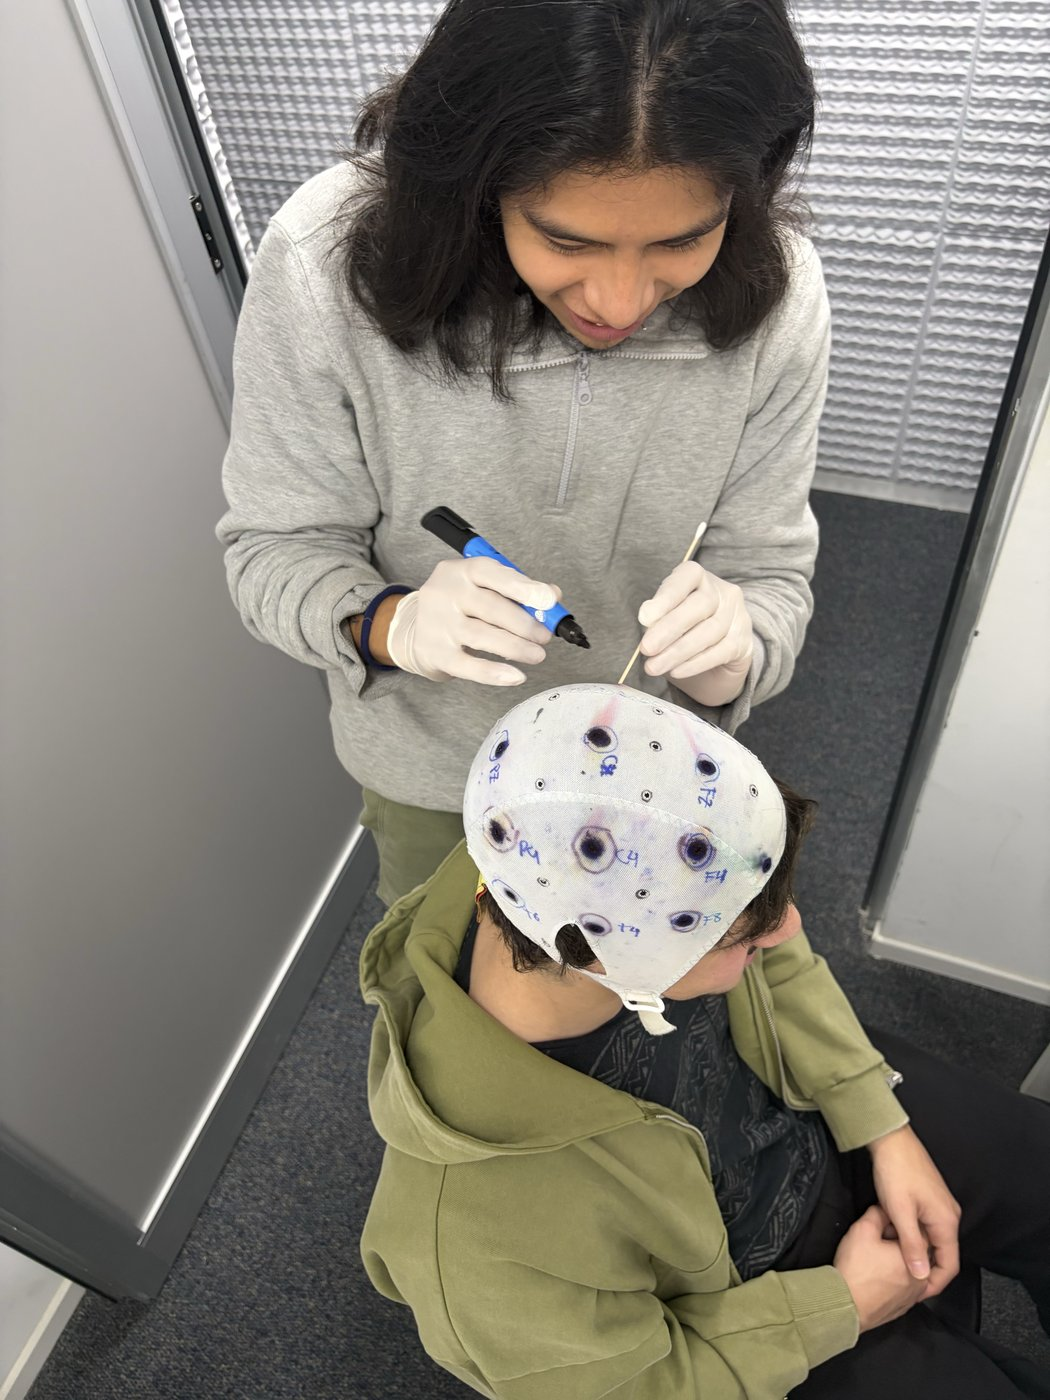
\includegraphics[height=0.54\textheight]{foto_electrodos_v3.jpg}\\[2pt]
      {\scriptsize\color{muted} Foto del procedimiento propio (OpenBCI); no es el EEG de sueño analizado.}
    \end{column}
  \end{columns}
\end{frame}

% ---------- 7. METODOS CONDUCTUALES -----------------------------------------
\begin{frame}{Tarea de palabras: recuerdo formal vs.\ recuerdo semántico}{Métodos conductuales}
  \begin{itemize}\setlength\itemsep{5pt}
    \item En TR/TS cada sujeto trabaja con 20 \textbf{asociaciones} palabra rara--definición.
    \item Dos puntajes independientes por sujeto:
      \begin{itemize}\setlength\itemsep{2pt}
        \item \textbf{Palabra objetivo:} coincidencia \emph{formal} exacta (normalizando mayúsculas/acentos).
        \item \textbf{Definición:} scoring \emph{semántico} binario, documentado ítem por ítem.
      \end{itemize}
    \item Análisis \textbf{descriptivo}: la condición sueño tiene \textbf{$n=1$}.
  \end{itemize}
  \vskip3pt
  \begin{block}{Por qué dos puntajes}
    Recuperar la \textbf{forma exacta} de una pseudopalabra es más exigente que recuperar su \textbf{significado}: separa la dificultad de la tarea.
  \end{block}
\end{frame}

% ---------- 8. METODOS EEG ---------------------------------------------------
\begin{frame}{EEG con MNE: filtrar antes de medir y revisar la calidad de canal}{Métodos de señales fisiológicas}
  \begin{columns}[T,onlytextwidth]
    \begin{column}{0.58\textwidth}
      \begin{itemize}\setlength\itemsep{4pt}
        \item Lectura BrainVision con \textbf{MNE} (10 canales, 250 Hz).
        \item \textbf{Filtros} antes del análisis: \textbf{notch 50 Hz} + \textbf{pasa banda 0.3--35 Hz} (quita deriva/DC y ruido).
        \item \textbf{Épocas de 30 s} sin solapamiento, alineadas 1:1 con el scoring.
        \item Canales centrales \textbf{C3/C4}; potencia por banda con Welch.
      \end{itemize}
    \end{column}
    \begin{column}{0.42\textwidth}
      \begin{block}{Control de calidad}
        \footnotesize
        \begin{tabular}{lrl}
          \toprule
          Canal & std (uV) & Estado\\
          \midrule
          C3 & 28 & \textbf{\color{good}OK}\\
          C4 & 513 & \textbf{\color{warn}descartado}\\
          \bottomrule
        \end{tabular}\par\vskip4pt
        C4 tenía artefactos y saturación: se \textbf{descarta} y se analiza \textbf{C3}.
      \end{block}
    \end{column}
  \end{columns}
\end{frame}

% ---------- 9. SCORING -------------------------------------------------------
\begin{frame}{Scoring de sueño: lectura asumida hasta sueño profundo (S3/SWS)}{Códigos y fases}
  \begin{columns}[T,onlytextwidth]
    \begin{column}{0.46\textwidth}
      \footnotesize
      \begin{tabular}{cl}
        \toprule
        Código & Fase\\
        \midrule
        0 & Vigilia / transición\\
        1 & S1 (sueño liviano)\\
        2 & S2 (sigma / complejos K)\\
        3 & \textbf{S3 / SWS} (ondas lentas)\\
        \bottomrule
      \end{tabular}
      \vskip6pt
      \normalsize Descenso NREM consecutivo \textbf{0$\to$1$\to$2$\to$3}, en épocas de 30 s.
      \vskip4pt
      \begin{minipage}{0.95\linewidth}
        {\scriptsize\color{muted} Scoring descriptivo, no clínico. Confirmar clave oficial si la cátedra la solicita.}
      \end{minipage}
    \end{column}
    \begin{column}{0.54\textwidth}
      \begin{block}{Qué implica}
        \begin{itemize}\setlength\itemsep{2pt}
          \item Se llegó a \textbf{S3/SWS}, la fase clave para la consolidación.
          \item Protocolo previsto $\sim$90 min; registro útil analizado: \textbf{79.5 min}.
          \item Podía esperarse \textbf{S4} o \textbf{REM}, pero \textbf{no aparecen} en el scoring usado.
          \item Comparamos las fases por profundidad; el foco es \textbf{S3/SWS}.
        \end{itemize}
      \end{block}
    \end{column}
  \end{columns}
\end{frame}

% ---------- 10. RESULTADOS CONDUCTUALES -------------------------------------
\begin{frame}{Resultados conductuales: desempeño final y cambio TR$\to$TS}{Tarea de palabras}
  \begin{columns}[c,onlytextwidth]
    \begin{column}{0.62\textwidth}
      \centering
      
\includegraphics[width=\linewidth]{2026-06-11_memoria_scores_v1.png}
    \end{column}
    \begin{column}{0.38\textwidth}
      \footnotesize
      \begin{tabular}{llrrr}
        \toprule
        Suj. & Cond. & TR & TS & $\Delta$\\
        \midrule
        1 & Vig. & 0 & 0 & 0\\
        2 & Vig. & 10 & 14 & +4\\
        3 & Vig. & 1 & 1 & 0\\
        4 & Sueño & 15 & 17 & +2\\
        \bottomrule
      \end{tabular}
      \vskip6pt
      \begin{itemize}\setlength\itemsep{2pt}
        \item Sueño tuvo mayor \textbf{TS} final, pero ya partía alto.
        \item La mejora TR$\to$TS fue \textbf{+2}; el resultado es descriptivo.
      \end{itemize}
      \vskip3pt
      \claim{Compatible con la hipótesis, sin inferencia causal.}
    \end{column}
  \end{columns}
\end{frame}

% ---------- 11. HIPNOGRAMA ---------------------------------------------------
\begin{frame}{El dataset secundario recorrió un descenso NREM completo hasta S3/SWS}{Arquitectura del sueño: hipnograma}
  \centering
  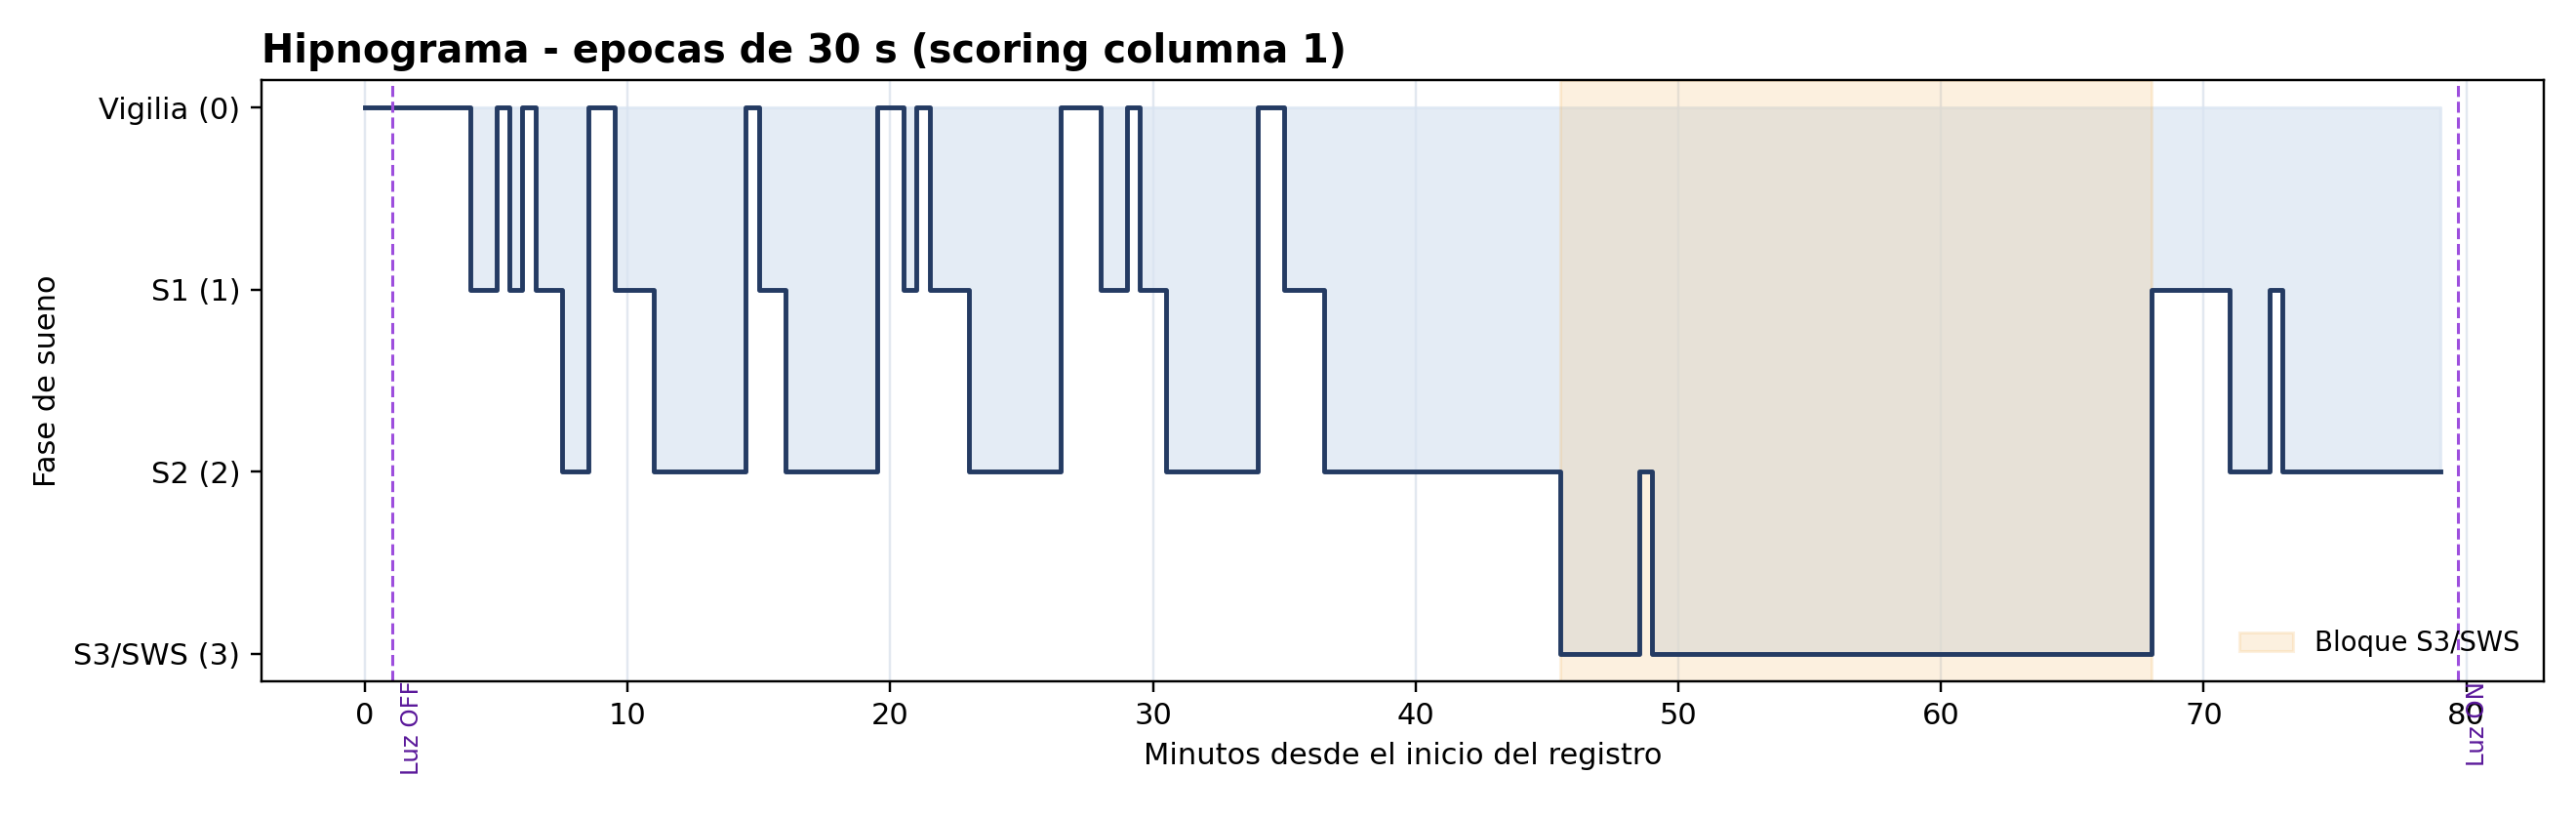
\includegraphics[width=0.96\linewidth]{2026-06-11_eeg_hipnograma_mne_v3.png}
  \begin{columns}[T,onlytextwidth]
    \begin{column}{0.5\textwidth}
      {\footnotesize $\bullet$ Latencia de sueño: \textbf{4 min} \quad $\bullet$ Latencia a S3: \textbf{45.5 min}}
    \end{column}
    \begin{column}{0.5\textwidth}
      {\footnotesize $\bullet$ Bloque S3/SWS sostenido: \textbf{45.5--68 min} \quad $\bullet$ Sin REM}
    \end{column}
  \end{columns}
\end{frame}

% ---------- 12. DISTRIBUCION DE FASES ---------------------------------------
\begin{frame}{Predomina el NREM, con casi 28\% del registro útil en sueño profundo}{Tiempo por fase y latencias}
  \begin{columns}[c,onlytextwidth]
    \begin{column}{0.56\textwidth}
      \centering
      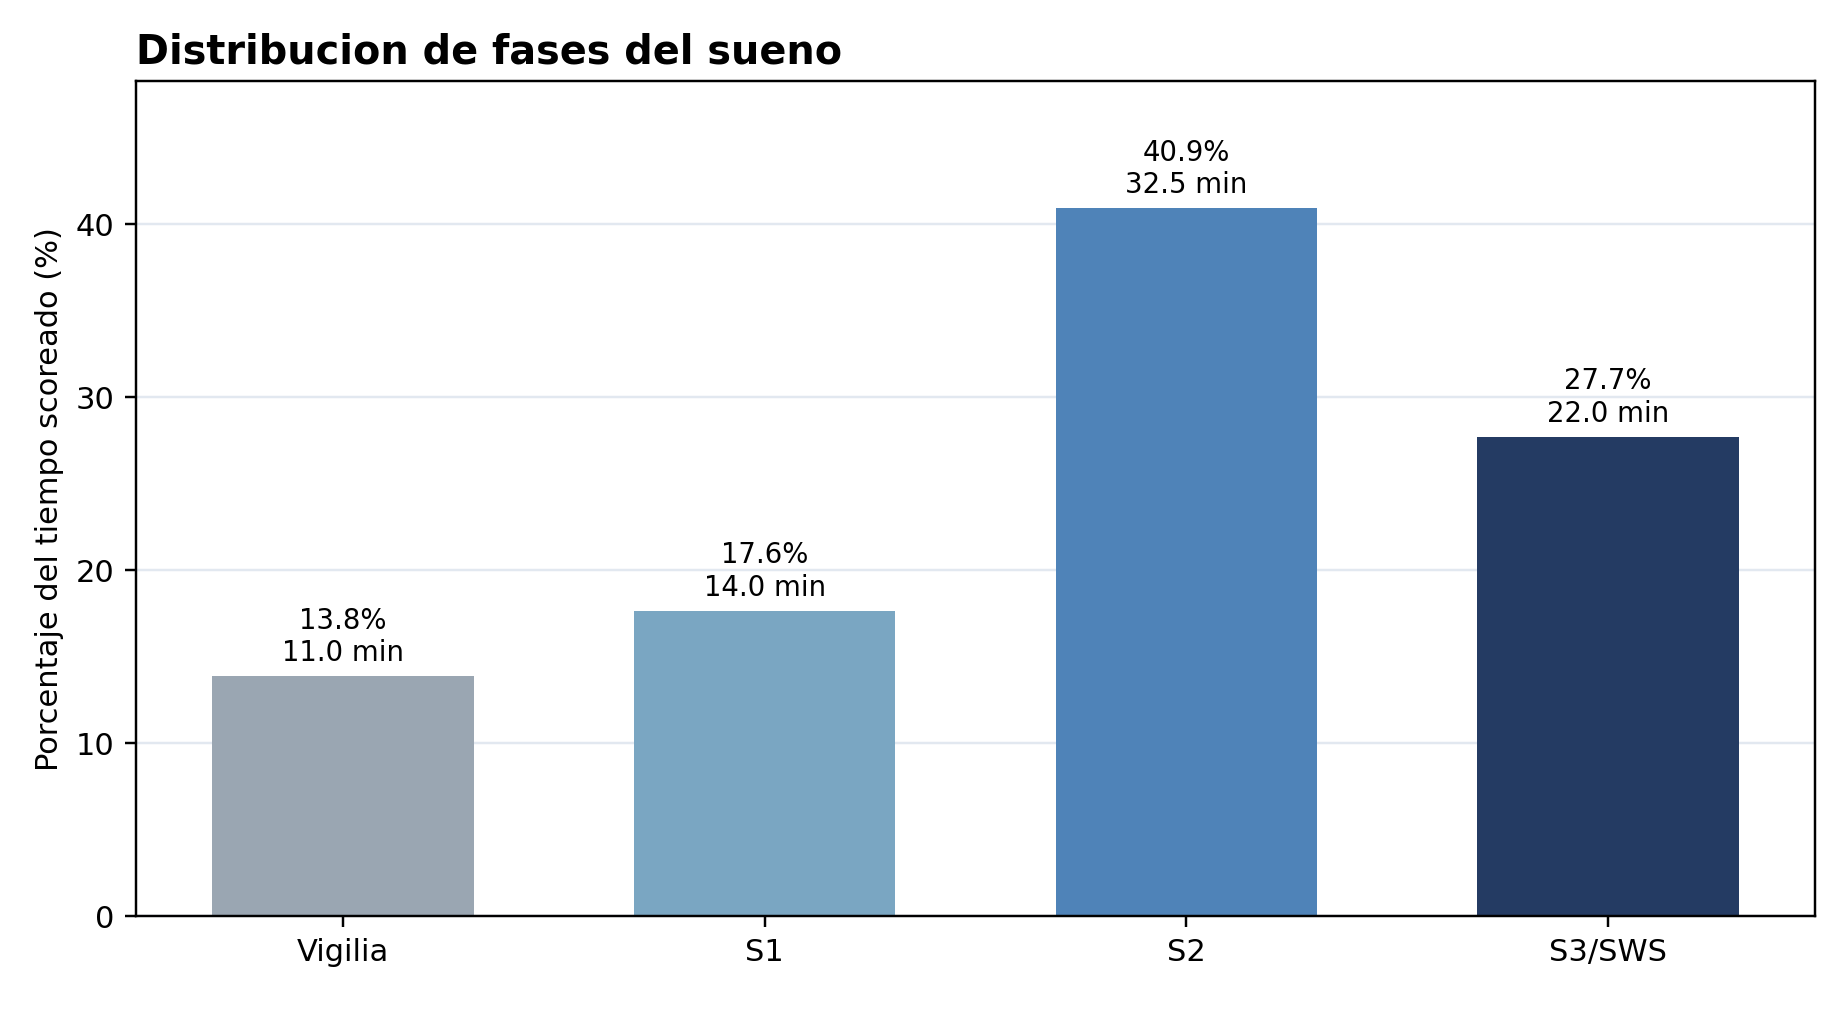
\includegraphics[width=\linewidth]{2026-06-11_eeg_porcentaje-fases_v3.png}
    \end{column}
    \begin{column}{0.44\textwidth}
      \begin{itemize}\setlength\itemsep{5pt}
        \item S2: \textbf{40.9\%} (32.5 min) -- la fase más larga.
        \item S3/SWS: \textbf{27.7\%} (22 min) -- sueño profundo presente.
        \item Vigilia 13.8\% + S1 17.6\%: sueño liviano/transición.
        \item Eficiencia de sueño: \textbf{86\%} del registro.
      \end{itemize}
      \vskip8pt
      {\footnotesize\color{muted} Dataset secundario BrainVision; registro útil analizado: \textbf{79.5 min}.}
    \end{column}
  \end{columns}
\end{frame}

% ---------- 13. POTENCIA POR BANDA ------------------------------------------
\begin{frame}{Delta crece hacia S3 y la banda sigma tiene su pico en S2}{Potencia por banda y fase (C3)}
  \centering
  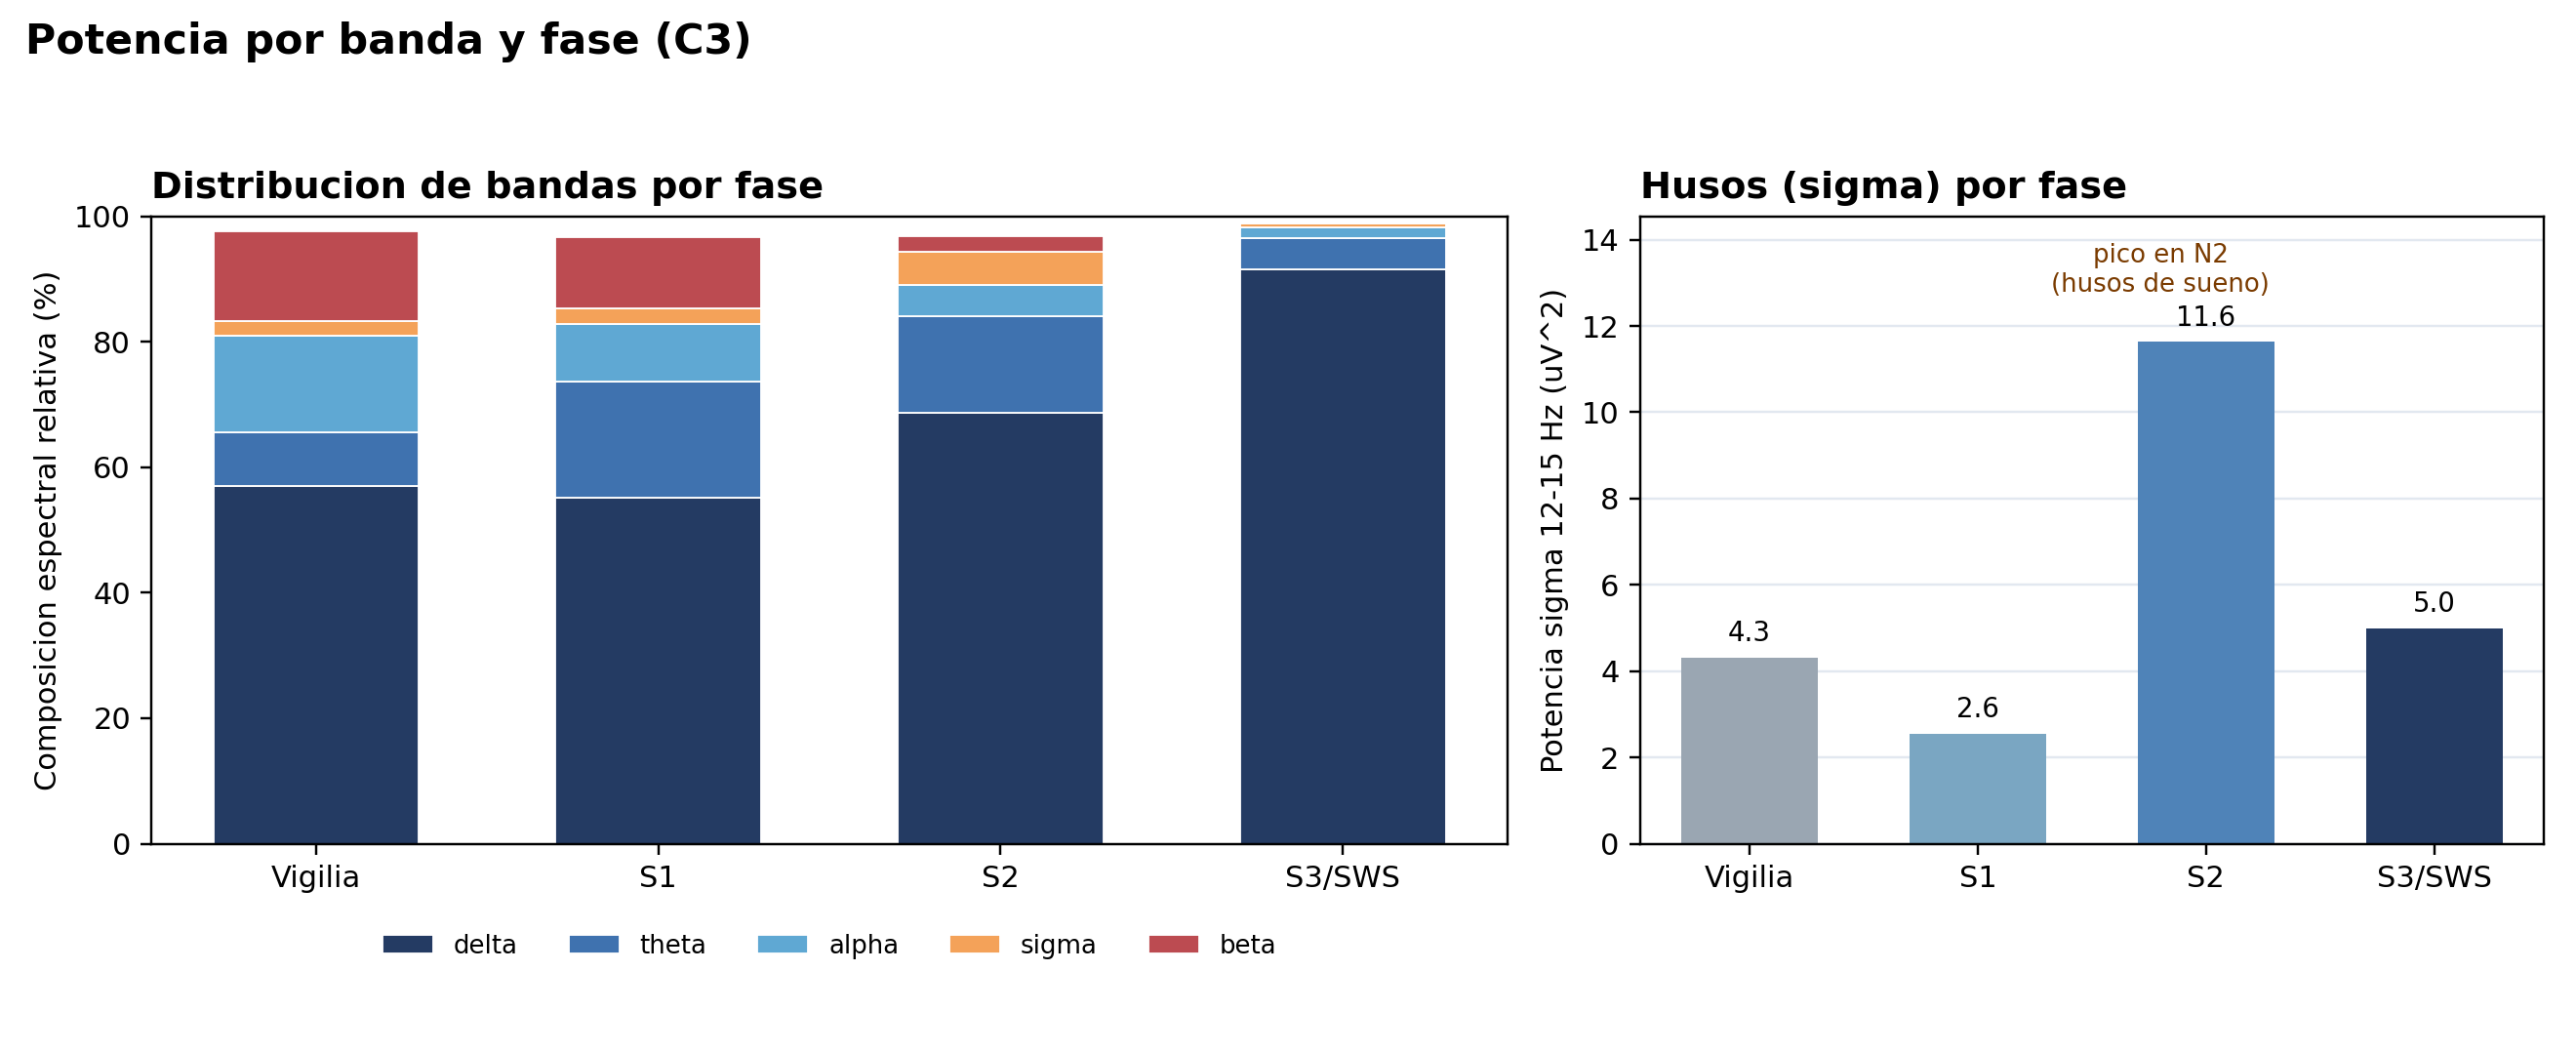
\includegraphics[width=0.82\linewidth]{2026-06-11_eeg_potencia-bandas-por-fase_v3.png}\\[3pt]
  {\footnotesize Delta relativa sube de 57\% (Vigilia) a \textbf{92\% en S3}; la sigma, \textbf{proxy compatible con husos}, es máxima en \textbf{S2}.}
\end{frame}

% ---------- 14. ESPECTROGRAMA + HUSOS/MEMORIA -------------------------------
\begin{frame}{Sigma y memoria: integramos el mecanismo, no inventamos una correlación}{Qué podemos y qué no podemos concluir}
  \begin{columns}[T,onlytextwidth]
    \begin{column}{0.55\textwidth}
      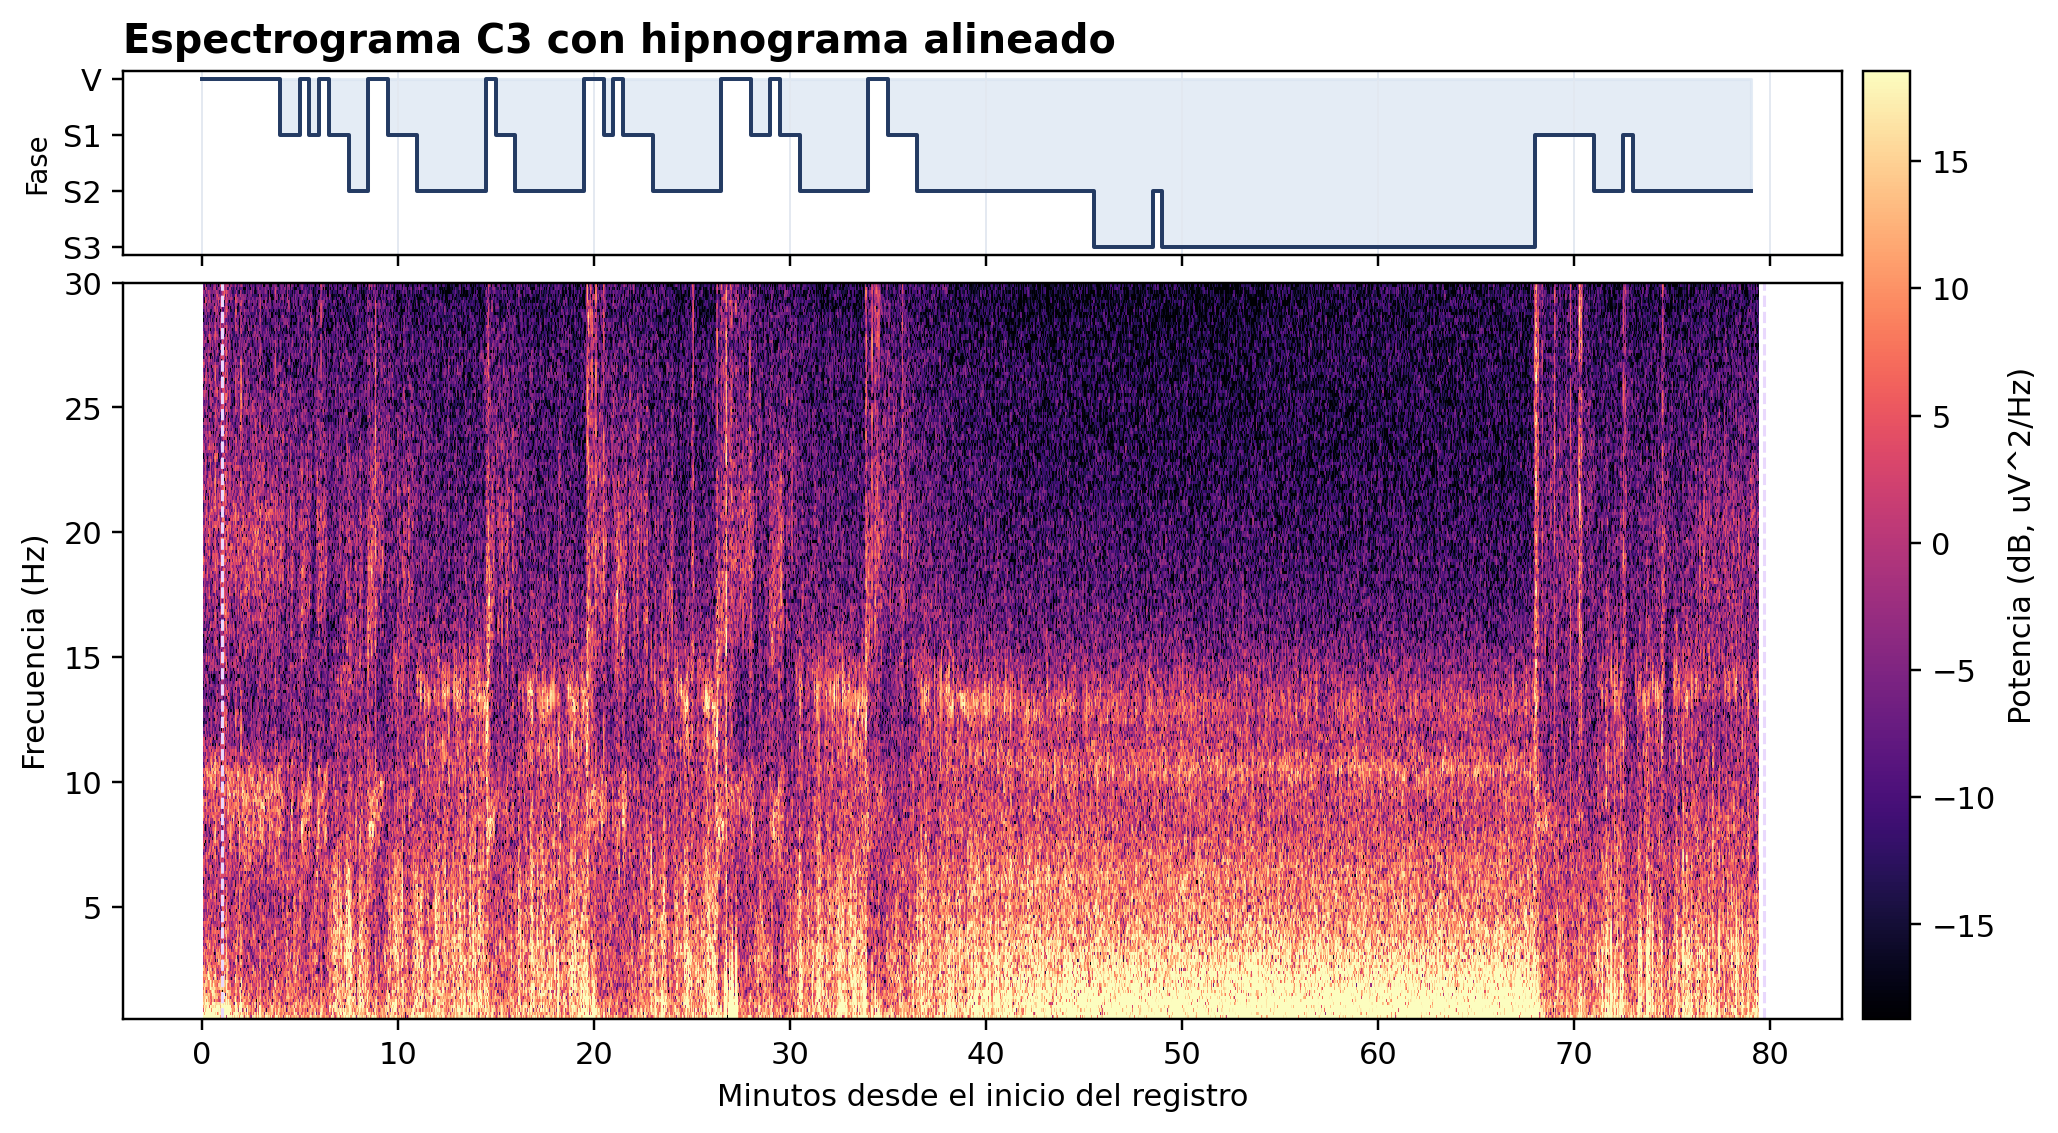
\includegraphics[width=\linewidth]{2026-06-11_eeg_espectrograma_c3-c4_mne_v3.png}\\[1pt]
      {\scriptsize\color{muted} El bloque S3 (45--68 min) concentra la potencia lenta.}
    \end{column}
    \begin{column}{0.45\textwidth}
      \begin{block}{Sí podemos decir}
        \footnotesize Hay potencia sigma compatible con husos en S2 y ondas lentas en S3: ritmos que la teoría liga a la consolidación.
      \end{block}
      \begin{alertblock}{No podemos decir}
        \footnotesize ``Los husos de \emph{este} EEG explican la memoria de \emph{esos} sujetos'': EEG y memoria son \textbf{fuentes distintas}.
      \end{alertblock}
      {\scriptsize\color{muted} Sigma = proxy; detector de husos = trabajo futuro.}
    \end{column}
  \end{columns}
\end{frame}

% ---------- 15. VARIABLES EXTERNAS ------------------------------------------
\begin{frame}{Por qué el sujeto propio pudo no dormir: variables que modulan el descanso}{Discusión de factores contextuales}
  \begin{columns}[T,onlytextwidth]
    \begin{column}{0.62\textwidth}
      \begin{itemize}\setlength\itemsep{2pt}
        \item \textbf{Cronotipo / Proceso C:} siesta 16:00 podría ir a contra-fase.
        \item \textbf{Café:} podría bloquear adenosina y subir latencia.
        \item \textbf{Estrés:} podría aumentar activación y dificultar conciliar.
        \item \textbf{Pantallas / luz:} podrían retrasar fase.
        \item \textbf{Ambiente/dispositivo:} laboratorio y electrodos incómodos.
      \end{itemize}
      \vskip6pt
      {\footnotesize\color{muted} \textbf{Variables plausibles}, no causas confirmadas.}
    \end{column}
    \begin{column}{0.38\textwidth}
      \centering
      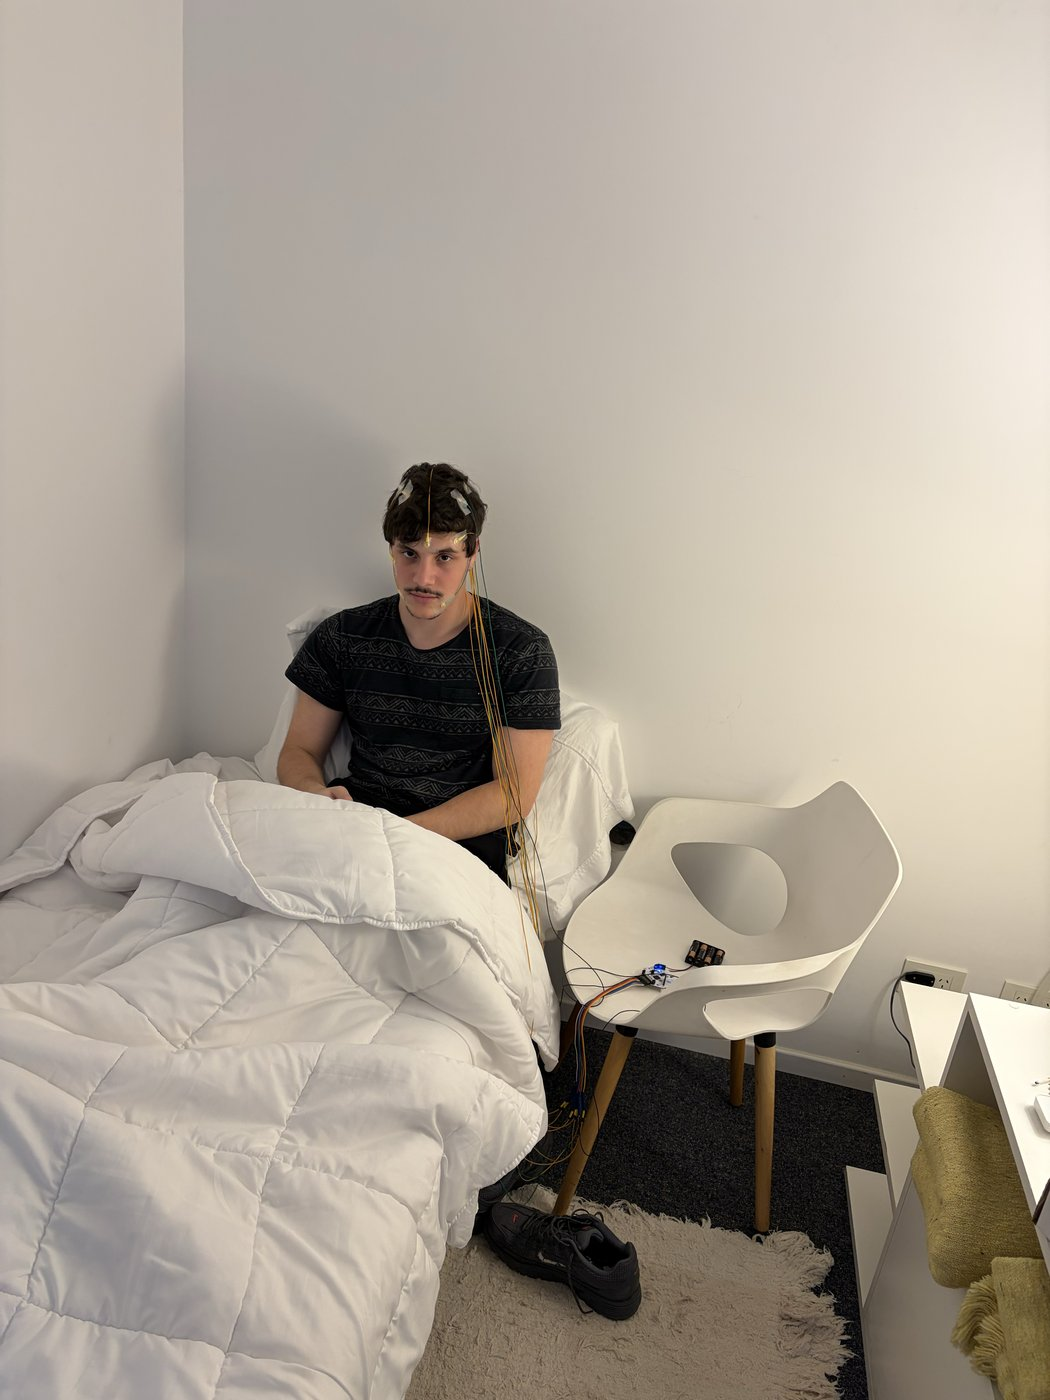
\includegraphics[height=0.48\textheight]{foto_pre-siesta-listo_v3.jpg}\\[2pt]
      {\scriptsize\color{muted} Sujeto propio listo para la siesta (OpenBCI).}
    \end{column}
  \end{columns}
\end{frame}

% ---------- 16. DISCUSION INTEGRADA -----------------------------------------
\begin{frame}{Discusión integrada: resultados, teoría y límites}{Cómo se sostiene el trabajo}
  \begin{columns}[T,onlytextwidth]
    \begin{column}{0.5\textwidth}
      \textbf{\color{navy}Lo que encaja}
      \begin{itemize}\setlength\itemsep{2pt}
        \item Mayor desempeño final en sueño y mejora TR$\to$TS descriptiva.
        \item Arquitectura NREM con SWS y potencia sigma elevada en S2.
        \item Coherente con consolidación activa + homeostasis sináptica.
      \end{itemize}
    \end{column}
    \begin{column}{0.5\textwidth}
      \textbf{\color{warn}Limitaciones}
      \begin{itemize}\setlength\itemsep{2pt}
        \item $n=1$ en sueño; sin estadística.
        \item EEG y memoria de \textbf{sujetos distintos}.
        \item El registro no llegó a S4 ni REM.
        \item Sigma como proxy, sin detector de husos.
      \end{itemize}
    \end{column}
  \end{columns}
  \vskip5pt
  \claim{Integramos el mecanismo de la materia sin sobre-afirmar lo que los datos no permiten.}
\end{frame}

% ---------- 17. CONCLUSION ---------------------------------------------------
\begin{frame}{Conclusión}{Respuesta directa a la pregunta}
  \begin{itemize}\setlength\itemsep{3pt}
    \item Compatible con la hipótesis: mayor desempeño final y mejora TR$\to$TS descriptiva en sueño.
    \item EEG secundario: NREM con sueño profundo y sigma elevada en S2.
    \item Apoyo \textbf{descriptivo/parcial}, no demostración causal: $n$ pequeño, fuentes separadas, sin S4/REM.
    \item El no-sueño del sujeto propio permite discutir cronotipo, cafeína, estrés, ambiente e higiene.
  \end{itemize}
  \vskip6pt
  \claim{El sueño aparece como un aliado de la memoria declarativa; lo afirmamos con la cautela que los datos exigen.}
\end{frame}

% ---------- APENDICE ---------------------------------------------------------
\appendix
\begin{frame}{Apéndice -- PSD promedio por fase (C3)}{Material de respaldo}
  \centering
  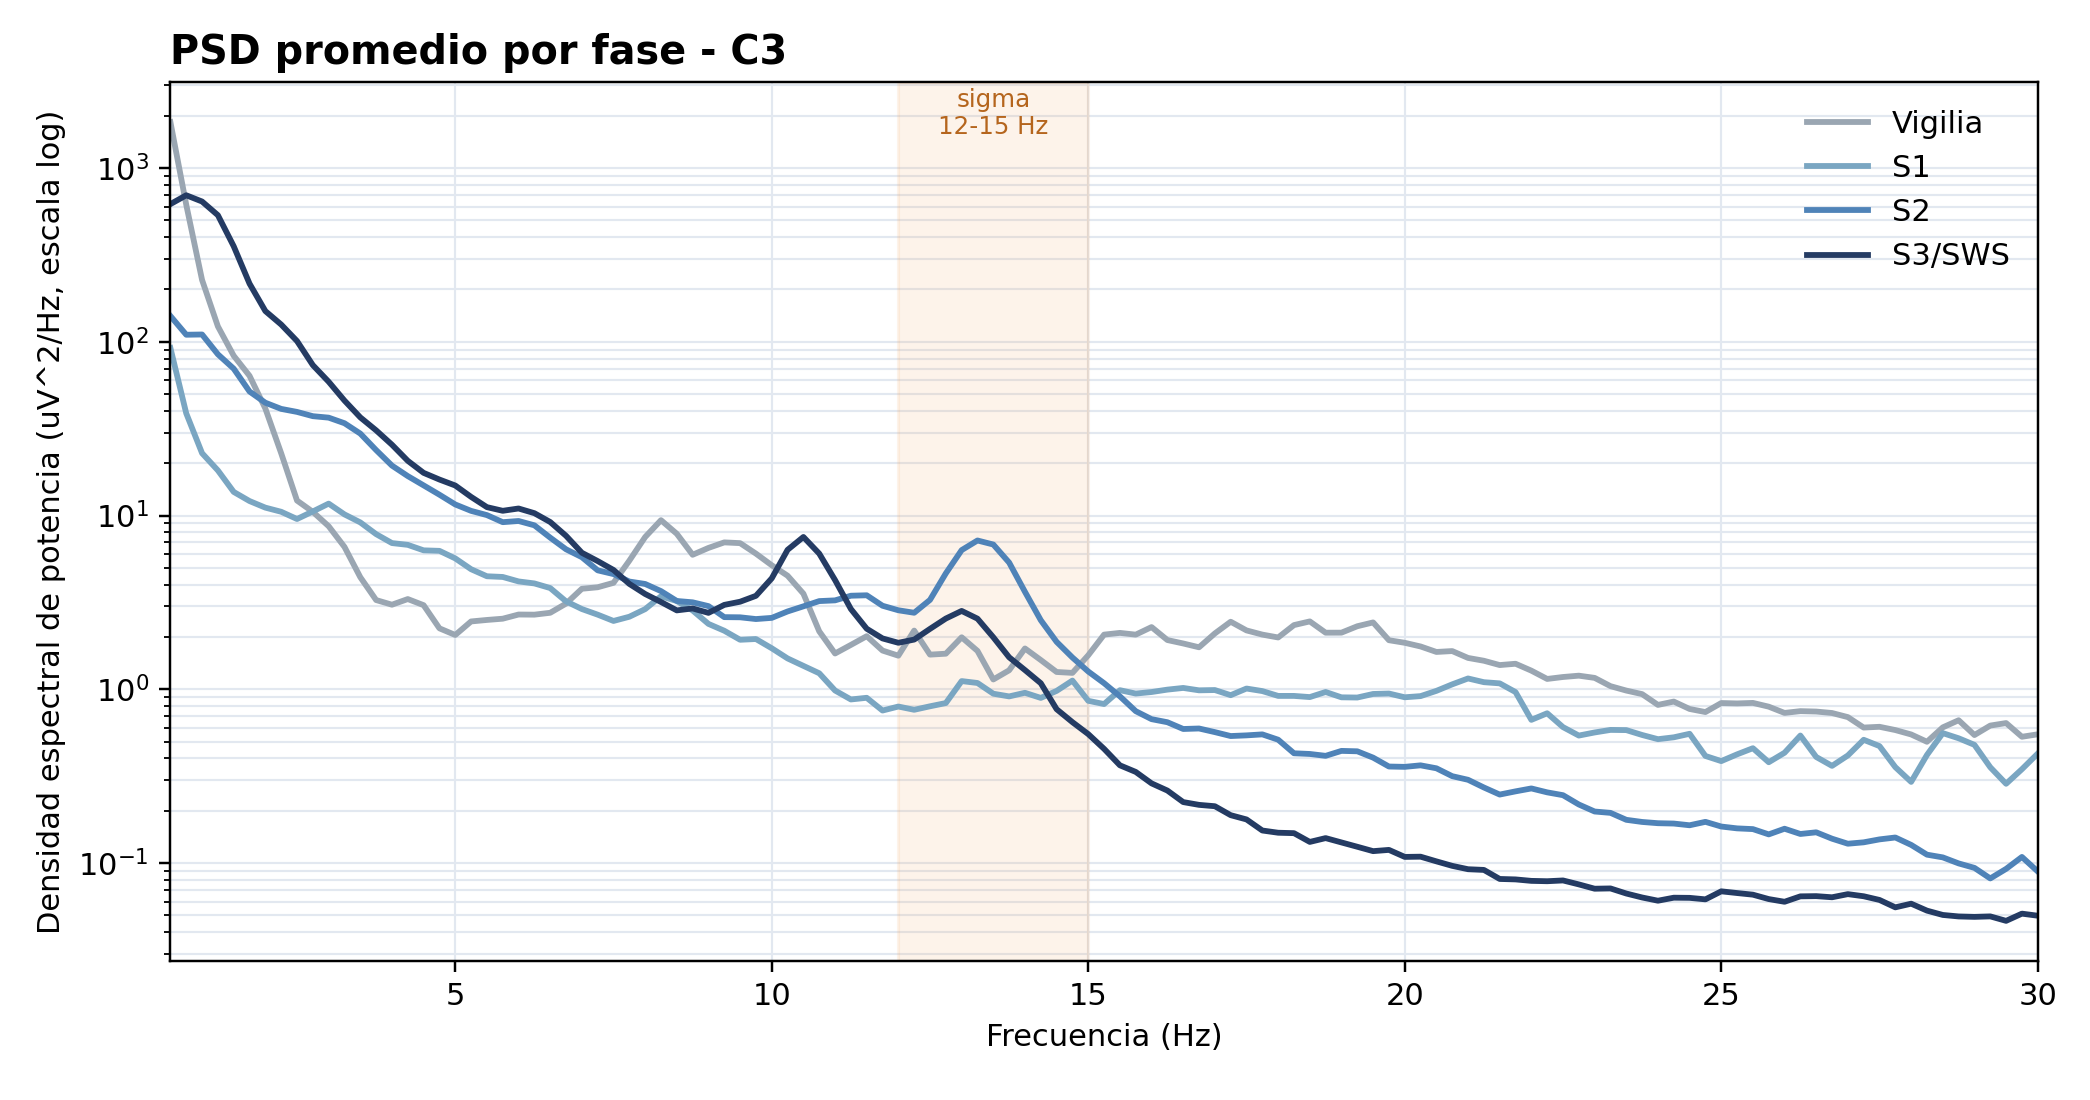
\includegraphics[width=0.66\linewidth]{2026-06-11_eeg_psd-por-fase_v3.png}\\[2pt]
  {\footnotesize En S2 se aprecia un ``bump'' de sigma en 12--15 Hz compatible con husos; S3 muestra la mayor potencia lenta.}
\end{frame}

\begin{frame}{Apéndice -- Ficha técnica del análisis}{Reproducibilidad}
  \footnotesize
  \begin{itemize}\setlength\itemsep{3pt}
    \item \textbf{Señal:} BrainVision, 10 canales, 250 Hz; canal usado \textbf{C3} (C4 descartado por artefactos).
    \item \textbf{Filtros:} notch 50 Hz + pasa banda 0.3--35 Hz (FIR).
    \item \textbf{Épocas:} 159 de 30 s, sin solapamiento, alineadas al scoring (1.ª columna).
    \item \textbf{Bandas:} delta 0.5--4, theta 4--8, alfa 8--12, sigma 12--15, beta 15--30 Hz.
    \item \textbf{Fases observadas:} Vigilia, S1, S2, S3/SWS (sin S4 ni REM).
  \end{itemize}
\end{frame}

\end{document}
